\section{Methods and Implementation}

\subsection{Data Collection}

The data collection system was written in Python, using the srcomapi \cite{srcomapi} module for interacting with the speedrun.com. The srcomapi module encapsulates the structures and endpoints of the REST API and allows an easier developer experience. The responses from the REST API were stored in a SQLite database via the requests\_cache \cite{requests_cache} module. The requests to the REST API were only processed if the response code was 200 (a successful request). Any other errors from the request— apart from a Not Found error— triggered repeated requests until the original request was successful. The requests were repeated to automate as much of the collection process as possible. Likewise, responses were cached to reduce the effect of repeated requests on the rate limit of the API. Subsequent requests could be fulfilled using a cached response instead of sending redundant requests that were previously successful. Individual 'feature` classes were responsible for processing and storing a single type of data, using composition for utility classes such as requesting logic. The collection system wrote directly to a raw data directory to enable distribution for further research and analysis. 


To ensure that all the collected data was accurate, all endpoints that allowed filtering by date set a maximum date of January 1st, 2023. This was done throughout all the data in this project, as to ensure the veracity of data. The date filtering option was not available for all endpoints so inaccuracies were present in the collected data. These inaccuracies were adjusted during the cleansing of the data. 


Games metadata was initially retrieved using a bulk method, which provided a large amount of games with limited metadata. Subsequent requests to the games endpoint with each games' internal ID expanded upon the limited metadata. However, this endpoint did not contain information about the total number of runs, or the number of users and guests that have played a game. To collect this information, the collection system scraped a statistics webpage. For certain games this webpage was not functional, so these values were set to a special value to be filtered out or supplemented during the cleaning process. All games metadata was written to a single CSV file.


The leaderboard endpoint of the REST API can be filtered by game ID, category ID, and level ID. The collector class iterated through the leaderboards for each combination of game, category, and level and stored all unique user IDs in those leaderboards. Another collector class then wrote the personal best(s) for every user in every leaderboard of a game to a corresponding file in the \texttt{games} directory. Due to the method of collection, games with non-functional leaderboards could not be collected. The videogame Subway Surfers could not be collected at this stage as it did not have a single functional leaderboard. This is a notable example as it is reported to have the largest number of runs and users on speedrun.com \cite{subway_surfers}. Therefore, Subway Surfers is not present in further processes or analysis. This technique was used to collect information on the games that users play as there is no direct method to obtain a list of all user IDs. The individual runs of all the users, and metadata about each user were also collected using the user IDs from the previous method. Only verified runs were collected by filtering the requests by the run status as 'verified`. The individual runs of each user were saved to a corresponding file in the \texttt{users} directory. All user metadata was written into a single CSV file.


All the collected data was tested to ensure that the data was accurate. Specifically, the metadata, user runs data, and leaderboard data were tested by comparing the statistics of the collected data to the About page of speedrun.com. This page lists the amount of runs, users, and games on the website. The user runs and leaderboard data were also tested by comparing users in the dataset and their corresponding webpage. This verified that the information was correct. These tests corroborated each other determining that the data is mostly correct prior to cleansing and transformation.

\vspace{-10pt}
\begin{figure}[h]
  \centering
  \begin{subfigure}{0.5\linewidth}
    \centering
    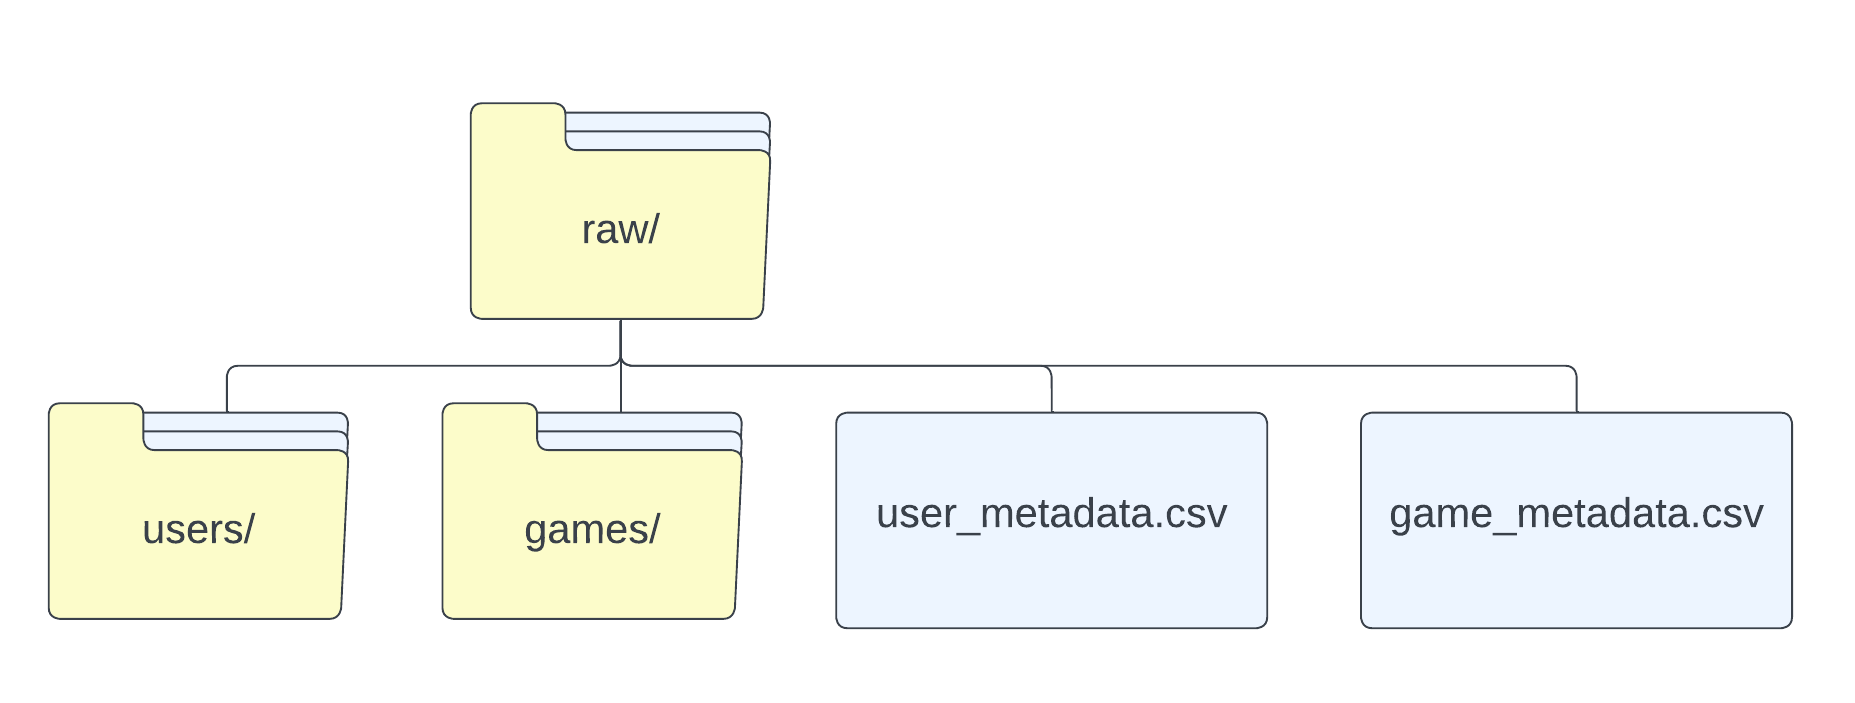
\includegraphics[width=\linewidth]{images/data-collection.png}
    \caption{Raw data.}
    \label{fig:figure1}
  \end{subfigure}
  \hspace{0.05\linewidth}
  \begin{subfigure}{0.4\linewidth}
    \centering
    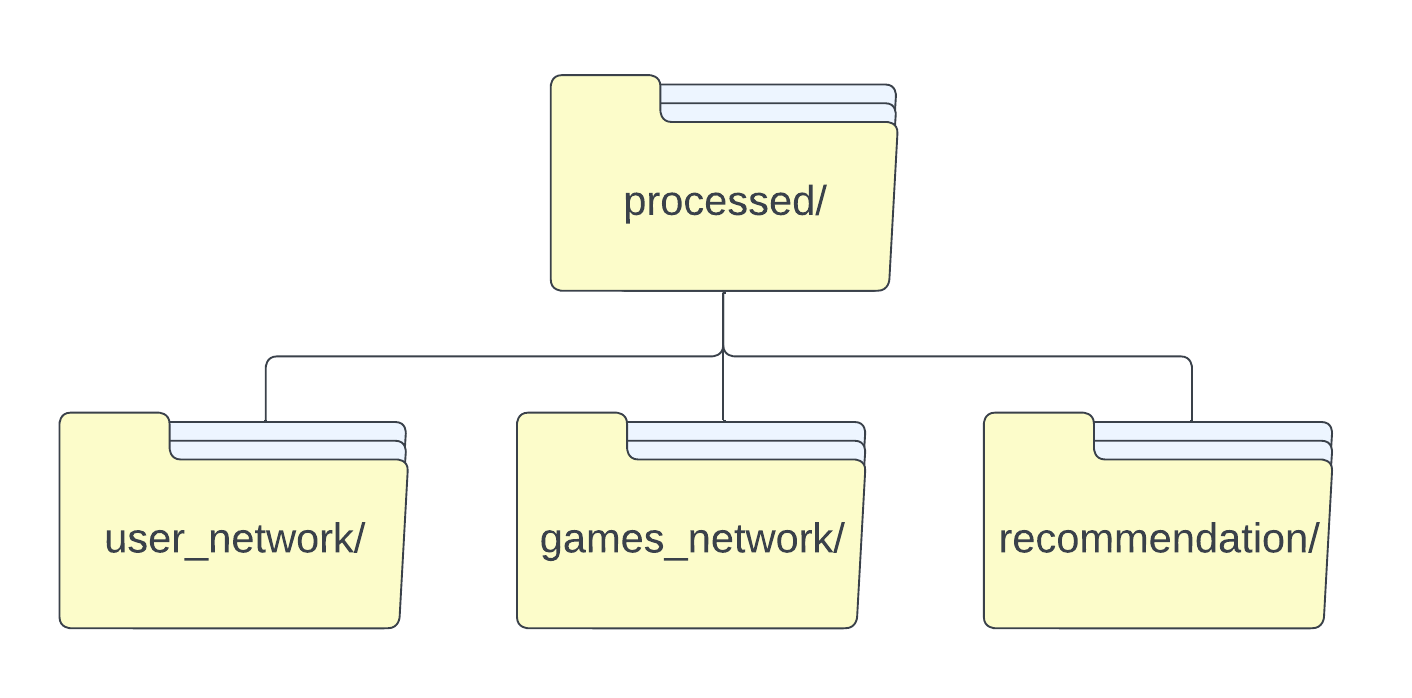
\includegraphics[width=\linewidth]{images/data-cleaning-transformation.png}
    \caption{Cleaned and transformed data.}
    \label{fig:figure2}
  \end{subfigure}
  \caption{Layout of data.}
  \label{fig:figures}
\end{figure}
\vspace{-20pt}

\subsection{Data Cleansing}

\renewcommand{\arraystretch}{1.2}
\begin{table}[h]
    \centering
    \begin{tabular}{|*{3}{D|}}
        \hline
        \textbf{Feature Name} & \textbf{Data Type} & \textbf{Example} \\ \hline
        game\_id & String & ``k6q4rqzd'' \\ \hline
        game\_name & String & ``Seterra'' \\ \hline
        game\_created\_date & Datetime & 2018-09-27T08:29:37Z \\ \hline
        game\_release\_date & Date & 1997-01-01 \\ \hline
        game\_developers & Comma-separated string & ``4eppvoer,ne410dem'' \\ \hline
        game\_num\_categories & Integer & 29 \\ \hline
        game\_num\_levels & Integer & 903 \\ \hline
        game\_num\_runs & Integer & 61962 \\ \hline
        game\_num\_users & Integer & 7168 \\ \hline
        game\_num\_guests & Integer & 36 \\ \hline
        user\_id & String & ``e8e52yp8'' \\ \hline
        user\_signup\_date & Datetime & 2017-12-08T03:05:55Z \\ \hline
        user\_location & String & ``br'' \\ \hline
        user\_num\_games & Integer & 2 \\ \hline
        user\_num\_runs & Integer & 5 \\ \hline
        user\_games & Comma-separated string & ``j1lq8v6g,m1zklz1''\\ \hline
    \end{tabular}
    \caption{Features of user and game metadata.}
    \label{tab:my_label}
\end{table}

Due to the method of collection, there were some remaining inaccuracies in the games metadata. Some features of this data were clean (\texttt{game\_id} and \texttt{game\_name}), as they were required to be a valid game on speedrun.com. All other features of this data set were either incomplete or inaccurate. The \texttt{release\_date} and \texttt{created\_date} features contained date values in different formats and had many null values. These features were converted to a single format and the null values were separated into another data source. The date features were also filtered so the games with created or release dates after January 1st, 2023 were removed. This step removed 786 games. The \texttt{num\_categories} and \texttt{num\_levels} features were collected during the bulk collection phase and contained no invalid values. In contrast, the \texttt{num\_runs}, \texttt{num\_users}, and \texttt{num\_guests} fields contained purposely invalid values from the collection phase (specifically -999) to indicate that the information could not be collected. These values were either updated individually or removed depending if the correct information could be collected. This removed a further 803 games. In total 1,589 games were removed during cleaning.


The leaderboard data was cleaned by filtering the raw data using the game IDs from the cleaned games metadata step. Furthermore, games were removed if they had no runs or users. This further reduced the number of games present in the leaderboard data from 31,405 games to 30,433. 


The user metadata was incredibly accurate for the number of users in the dataset, but still contained invalid values. All \texttt{user} values were accurate as they are the internal ID for each user. Some users could not be found by the REST API, so their \texttt{signup\_date} was left as null. These values were removed to have a completely accurate dataset of active users and their sign-up dates. This step removed 74 users. The \texttt{signup\_date} feature was then filtered so that no users past January 1st, 2023 were considered for the analysis. This step removed 5,622 users. The \texttt{num\_games} and \texttt{games} fields were collected from the previously stored leaderboard data, and the location data contained no invalid values was previously cleaned when removing the null \texttt{signup\_date} values. The \texttt{num\_runs} feature was collected for a subset of all active users, so this was the final size of the user metadata data set. The cleaning process removed 8,121 users, resulting in complete information for 332,897 active users.


Overall, this step was incredibly straightforward, and the only issue encountered was games with non-functional leaderboard endpoints. The cleaned data was then the input to the data transformation stage. The transformation stage aims to prepare the cleaned data for analysis and machine learning applications.

\subsection{Data Transformation}

To fulfil the aims of the project, the data must be formatted for further analysis. The community detection processes require graphs with suitable nodes and edges. The game recommendation system requires data that is easy to compare both items and users with each other. Each piece of transformed data was written to a separate \texttt{processed} directory to identify which data is the result of analysis and not collection.


Two graphs were created from the cleaned data to analyse using both exploratory and community detection methods. First, a game-game network where nodes are game IDs, and weighted edges that represent the number of users that appear in a pair of games' leaderboards. The data source for this graph was the list of personal bests for each user in the data set. A transformation function iterated through each game in the \texttt{games} directory and tallied the number of users that appeared in a pair of games' leaderboards. This created a list of edges for the game-game network. Self-loops were removed at this stage, and pairs of games with zero shared users were not recorded. These edges were stored in a tab separated values (TSV) file, which is the default input format for graph analysis tools like Gephi. The game-game graph was tested by selecting a random sample of connected games, and determining if the edges between these games were valid in the list of all user runs.


The second graph is a user-game network with both games and users as nodes, and an edge exists if a user has played a game. The data source for this graph was the user metadata CSV which contained the game IDs of each game a user has played in a comma separated list. Each individual game ID was extracted from the comma separated list and formatted so that an individual entry was a single user ID and a single game ID. This is an edge list for a bipartite user-game graph, which was stored in a similar TSV format. These edges did not have weights, as the frequency of the number of runs a user has submitted for a single game was not collected until this analysis was completed. Similar to the game-game graph, the accuracy of the user-game graph was tested by selecting a random sample of users, and checking if the list of verified runs was the same as the neighbours of the user-game graph. 


The transformed data for the recommendation system used the same data source as the bipartite user-game network. Similarly, each game ID was extracted from the comma separated list of games. These game IDs were formatted so that a single entry was a user ID, followed by a game ID, and a binary variable representing if a user had played that game. This list of each user ID and game ID was then pivoted to create a sparse matrix $M$ of size $n_{\text{users}} \times n_{\text{games}}$. This matrix records if a user $i$ has played a game $j$ with $M_{ij} = 1$, and $M_{ij} = 0$ if not. The dot product of $M$ and $M^T$ produces the cosine similarity matrix of $M$. Unfortunately, if the whole data set was included in this process, it would require over 32 GB of memory to store a single matrix. Therefore, a smaller sample of users was chosen to create the recommendation system. Two samples were taken: one containing a number of the top users ranked by the number of games played, and another of a random sample of users. Each sample was split into a training and test splits, with an 80:20 train-to-test ratio. The first sample contained 5600 users after splitting the data, resulting in 23,930 games in the similarity matrix. The second sample contained 16,000 users after splitting the data and contained only 9,650 games. For further analyses, the sample of top users was chosen to include the maximum number of games possible in the final recommendation system.

\vspace{-10pt}
\begin{figure}[h]
    \centering
    \hspace*{-1cm}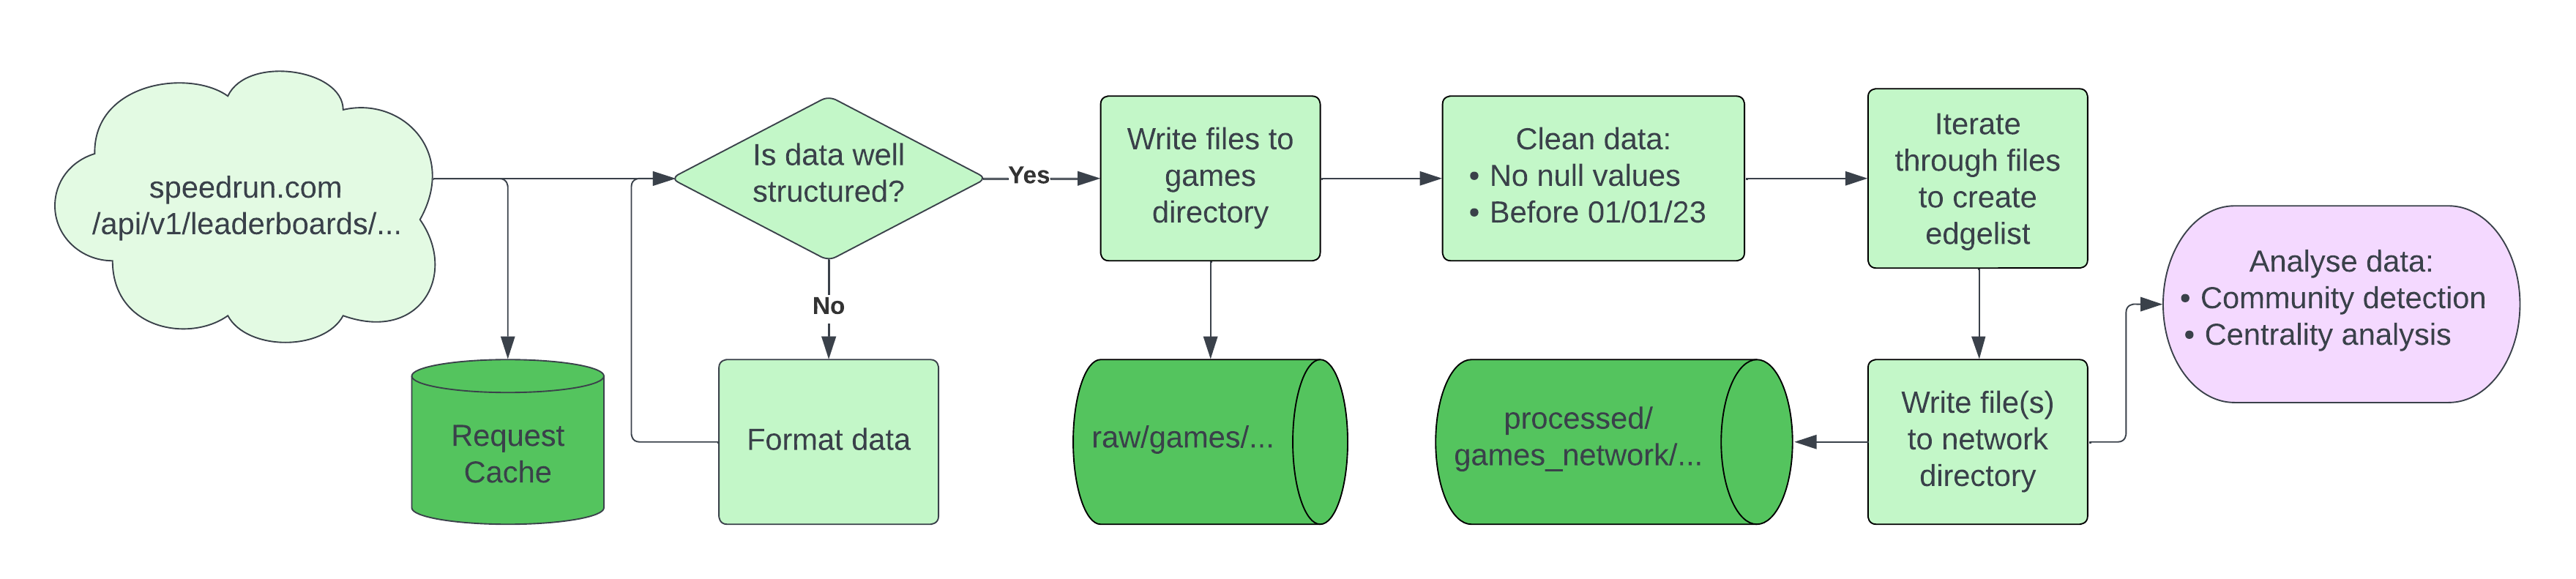
\includegraphics[width=1.1\linewidth]{images/leaderboard-process-2.png}
    \caption{Flow from data source to analysis for the game-game network using leaderboard data.}
    \label{fig:my_label}
\end{figure}
\vspace{-10pt}

\subsection{Methods of Data Analysis} 

From prior research, the Louvain, Infomap, and Clauset-Newman-Moore community detection algorithms were chosen to run on the game-game and user-game networks. Only two of these algorithms (Louvain and Clauset-Newman-Moore) were implemented in the networkx module for Python. The implementation of Infomap was taken from the cdlib module. A secondary version of the Louvain algorithm was also necessary to run on bipartite networks. This secondary version was implemented in the sknetwork module. The Louvain algorithm has two hyperparameters available: \texttt{resolution} and \texttt{threshold}. Similarly, the Clauset-Newman-Moore algorithm accepted hyperparameters of \texttt{resolution}, \texttt{cutoff}, and \texttt{best\_n}. The Infomap algorithm did not accept any hyperparameters. To evaluate the performance of each of these methods, modularity, coverage, and performance were measured.


Two different methods of recommendation systems are used to create recommendations for the games of speedrun.com: content and collaborative filtering. These methods rely on assigning a similarity value between comparable items. 


The first method, collaborative filtering, uses the similarity between users to define which games to recommend. The formula for similarity between users is the Jaccard index, which measures the similarity between two sets by the ratio between their intersection and union. In this context, the two sets are the games that two users have played. The Jaccard index has been modified to use the total number of games available instead of the union of both sets of games. This was done to improve the precision of the recommendations and to not always recommend the most popular games. The Jaccard index was chosen as it directly measures the similarity between sets of games — the only data we have for each user's preferences. Due to the nature of the collaborative filtering method it cannot be evaluated via a train/test split. The users that are part of the test split are not in the train split, and cannot have a similarity metric to the users in the training data.


The content filtering method uses similarity between games to calculate recommendations. The cosine similarity matrix was used to calculate the similarity between a sample of games in the dataset, and provides a method to lookup all similarity values for a given game. There is a single hyperparameter for both recommendation systems, which is the number of output recommendations. The number of recommendations may change depending on the context of the use of the system. The content filtering method can be evaluated with both quantitative and qualitative methods, using metrics such as precision, recall, and F1-score. 
